%%%%%%%%%%%%%%%%%%%%%%%%%%%%%%%%%%%%%%%%%%%%%%%%%%%%%%%
%%% LATEX FORMATTING - LEAVE AS IS %%%%%%%%%%%%%%%%%%%%
\documentclass[11pt]{article} % documenttype: article
\usepackage[top=20mm,left=20mm,right=20mm,bottom=15mm,headsep=15pt,footskip=15pt,a4paper]{geometry} % customize margins
\usepackage{times} % fonttype
\usepackage{url}
\usepackage{graphicx}
\makeatletter         
\def\@maketitle{   % custom maketitle 
\begin{center}
{\bfseries \@title}
{\bfseries \@author}
\end{center}
\smallskip \hrule \bigskip }
\graphicspath{ {./images/} }

%%%%%%%%%%%%%%%%%%%%%%%%%%%%%%%%%%%%%%%%%%%%%%%%%%%%%%%%%%%%%%%%%%%%
%%% MAKE CHANGES HERE %%%%%%%%%%%%%%%%%%%%%%%%%%%%%%%%%%%%%%%%%%%%%%
\title{{\LARGE Machine Learning in Natural Language Processing: \newline Assignment 1}\\[1.5mm]} % Replace 'X' by number of Assignment
\author{Shifei Chen} % Replace 'Firstname Lastname' by your name.

%%%%%%%%%%%%%%%%%%%%%%%%%%%%%%%%%%%%%%%%%%%%%%%%%%%%%%%%%%%%%%%%%%%%
%%% BEGIN DOCUMENT %%%%%%%%%%%%%%%%%%%%%%%%%%%%%%%%%%%%%%%%%%%%%%%%%
%%% From here on, edit document. Use sections, subsections, etc.
%%% to structure your answers.
\begin{document}
\maketitle

\section{Data Exploration}

\subsection{Which features are most informative for the two data sets? Try to explain why some features are more informative than others.}

For German plural data set, the most three informative features are \verb|p6|, \verb|gender| and \verb|p5|, each of them has an infromation gain of around 0.7-0.8. In the English data set, \verb|p9|, \verb|p7| and \verb|p8| are the three features with highest information gain values, roughly around 0.18. So in both cases, we can see that the ultimate syllable played a much more significient role than other syllables, especially the coda. In addition, the gender in German is almost as informative as the code in the ultimate syllable. As we all know in English the past tense form of a verb mainly depends on the way it is spelled, for example for verbs ending in \verb|e| usually we just apply a single \verb|-d| to form its past tense form instead of the regular \verb|-ed| conjugation. Therefore the way a word is spelled largely decides how it should be pronounced hence it is not surprising to see the ultimate syllable has great influences on the past tense conjugation. For German I believe there is a similar case as the plural form depends on the ending of the noun and there are rules on how a masculine/feminine word should end. In other words, information gain correcly represented the grammatical rules in both the noun plural forms in German and the past tense form for verbs in English.

\section{Decision Trees}

\subsection{How accurate are the decision tree classifiers for the two data sets? Look at overall accuracy as well as precision and recall for specific classes.}

The decision tree classifier performed better for the plural forms of German nouns than the past tense forms for English verbs, regardless of which data set (training or test) it was validated on or whether it is pruned or unpruned. For a pruned decision tree tested on the test data, it has achieved 94.4\% in overall accuracy in German and a slightly lower 93.8\% accuracy in English. However its performance on individual classes were very different in these two languages. In German, most classes has a precision score over 0.9. Especially for the plural form \verb|en|, \verb|-| (unchanged plural form) and \verb|er| as their precision score were 0.98, 0.966 and 0.961, respectively. When we look at the recall score for German plural forms, those who has a precison score of 0.9 actually has a higher recall score in around 0.95, like class \verb|Uer| and \verb|Ue|, and some of those performed well in precison their recall score dropped to 0.9, except class \verb|-n| and \verb|-| as they performed equally well in both scores. Class \verb|s| and \verb|U| are the two that our decision tree classified had most difficult time to catch. Their recall scores were only 0.638 and 0.719.

In English, the pruned tree only has one single leaf \verb|REG|, which means it will always predict the verb to have a regular past tense form. But even its strategy is very naive it still achieved an accuracy of 93.81\% on our test data. The precision and recall score for \verb|REG| are 0.938 and 1. No other classes exist in the pruned decision tree.

\subsection{How does training error relate to test error? What is the effect of pruning?}

The results from the lab proved the theory that validating on the training data usually performs better than validating on the test data, even though it can't achieve 100\% perfect. All of the scores grew in my experiment no matter it was a pruned tree or an unpruned. It is also interesting to mention that in German, classes have a higher precision score than their recall scores still performs in the same pattern, as the other way around. In addition the recall scores for class \verb|s| and \verb|U| again are lower than other classes, even though they have improved from 0.7 to 0.85 now.

But there is an exception here. If we look at the pruned decision tree on English verbs, it remains the same accuracy, precision and recall scores no matter it is validated on the training data or the test data. Personally I believe this was caused by the fact that our decision tree has only one leaf after pruning. It does't really matter whether we are going to test our model on the whole 4400 instances (training data set) or doing the 10 fold cross validation (test data set)-it will always predict \verb|-ed|.

In many other cases, pruning makes the tree shallower at the cost of accuracy. In the German data set, pruning almost halved the tree from 25000 to 11500. In english if we apply the same method it will chop the tree from 7600 to only one leaf. At the same time, usually the accuracy drops 2-3\%. However in the case where it was tested on the test data set of English verbs, the decision tree classifier improved the accuracy by roughly 1\%.

In conclusion, I would say that we have generated a well-fitted decision tree for the plural forms of German nouns and an underfitted tree for the past tense forms of English verbs. Also, underfitting is the reason why validating on the training data set doesn't look like ``cheating'' on English verbs. It overgeneralized the data and didn't pick up all the distinctions in irregular forms hence the single \verb|REG| prediction can perform in the same way no matter what kind of data it is tested on.

\subsection{Can you make sense of the rules implicit in the trees? Consider especially the pruned tree for the English past tense data.}

After pruning the English past tense data has only one rule left, \verb|REG|, which is indeed the most common conjugation for English verbs. All of the other leaves and node were removed simply because their probabilities are much lower in our training data than the regular form. In the German noun tree I can see that the plural form is heavily related to the gender of the noun. For example if the noun is feminine then most likely its plural form is going to end in \verb|-en|.

In the unpruned tree I tried to find some sensible rules. Some of them I can relate to actual English grammar conjugation, such as \texttt{p8=aI \& p9=nd -> IRREG-aI-aU}, we can relate that to the verb \texttt{bind -> bond} or \texttt{find -> found}. The rule \texttt{p8=i: \& p9=p -> IRREG-i:-E+t} can be related to \texttt{keep -> kept}. There are some reasonable pathes in this underfitted tree, though most of the pathes I can't find the corresponding phonetic rules.

\section{K-Nearest Neighbor}

\subsection{How accurate are the nearest neighbor classifiers for the two data sets? Look at overall accuracy as well as precision and recall for specific classes.}

The nearest neighbor classifier got 91\% accuracy in both the German and English data set.

For German nouns, the class \verb|-|, \verb|U| and \verb|en| are the three that have the highest precison and recall score-all above 0.91 and 0.96. Then there are some classes which got approximately 0.8 in both scores such as \verb|Ue|, \verb|Uer|, \verb|e| and \verb|er|. Class \verb|s| is the one with lowerst scores. Our classifier only managed to achieve 0.718 in precision and 0.557 in recall.

The results is much worse if we take a look in English verbs. Most classes only got a precision score of 0.2-0.3 and a recall score of similar value. The regular past tense form is the only exception here. Class \verb|REG| got 0.961 in precision and 0.96 in recall. It explains why we can still have an accuracy of 91\% despite the poor performance in all the other classes.

So in both cases, we can see regular conjugations, which were also the most common class, were predicted better than the irrgular ones. Classes like \verb|en| in German and \verb|REG| have the highest score in both precision and recall while the scores of class \verb|s| in German and all the other \verb|IRREG*| classes are much lower.

\subsection{What is the effect of varying the $k$ parameter? Can you improve accuracy by removing less informative features?}

In the German noun plural form case, the accuracy goes down from 91\% to 90\% and stays there as we increase the k value. It looks like there is no overfitting if we set k to 1 as it has the highest accuracy. Also when $k=1$ I tried to remove all the other less informative features base on the information gain score ealier. The accuracy goes up by 1\% every time I remove one most irrelavant feature according to the information gain rankings until feature \verb|p2|. And from there I tried to increase the k value again but it didn't work as well. So in conclusion the best KNN classifier to the plural form of German nouns are the one featured \verb|p2|, \verb|p4|, \verb|p5|, \verb|p6| and \verb|gender|, with $k=1$. It got 94.1\% of accuracy.

In the English verb case that was a compeletely different story. I have increased the k value from 1 to 10. The corresponding accuracy dropped slightly from 91\% to 90.4\%, then from $k=3$ it jumped to 93\% and gradually climbs to 94\% until $k=6$. Then from $k=7$ to 10 the accuracy stablized at 93.9\%. The same pattern can be observed by removing less informative features as the accuracy goes to up 94.6\% until feature \verb|p8|. However the accuracy doesn't continue to go up when we combine these two methods together. It went all the way down as we increase the k value therefore I believe the best hyperparameter combination for the English data set is $k=1$ and the feature set only consists of \verb|p7|, \verb|p8|, and \verb|p9|.

So removing less informative features is an effective way to increase the accuracy in both cases. But whether it is effective by increasing the k value really depends on the data set. In the German case we have fewer categories to classifier so changing the $k$ value doesn't affect a lot, while in the English case there are altogether 42 different past tense forms so increasing the k value to 6 will increase the accuracy, if there is much noise in the data set. However after cleaning the noise, increasing the k value may not be effective any more.

\subsection{Does k-nearest neighbor perform better or worse than decision trees? Can you force the nearest neighbor classifier to behave like the pruned decision tree on the English past tense data?}

In the best cases, the k-NN algorithm performed slightly worse than the decision tree in the plural forms of German nouns, 94.1\% compared with 94.4\% in accuracy. It increased the accuracy from 93.8\% to 94.6\% in the past tense form of English verbs.

The nearest neighbor classifier can behave as pruning in the decision tree classifier. The pruned decision tree on the English past tense data only has one category \verb|REG| because the possibilities of all the other predictions are lower than the thredhold, which means they are not likely to happen. From the theory we know that the k-NN classifier will try to group the nearest $k$ neighbours together so if the data set has $N$ instances and we can set the $k$ value equal to $N-1$ then we are guranteened to have only one possible classification. In this situation the classifier has to think about all the other neighbours, which means it has to take everyone in the data set into consideration and is forced to make the most general prediction. Usually the k value doesn't has to be that large. In my practise if we set $k>=26$ on the English data set we will only get the \verb|REG| category, just like the pruned decision tree classifier.

\section{VG assignment}

\subsection{Describe how you ran these experiments and present the resulting learning curves, both in tabular and in graphical form. Report and discuss any interesting observations you made.}

In order to see the relation between the size of the data set and performance of the classifier, we need to apply a ``meta classifier'' before our classification algorithm to see the differences. I followed the video tutorial by YouTube user ``Rushdi Shams'' \footnote{\url{https://www.youtube.com/watch?v=ArU4x0Lnwi4}} who installed a filtered classifier with the filter ``Remove Percentage'' before the regular decision tree or k-NN classifier. After that by altering the parameter \verb|-p| we can choose how much training data by percentage we would like to randomly remove from our data set.

I have runned several experiments on the best performed classifiers with the German and the English data set. Below are the results.

\begin{table}[h]
    \begin{center}
        \caption{Classifiers' Performance with Different Sizes of Data}
        \label{tab:table1}
        \begin{tabular}{r|c|c|c|c}
            \textbf{Remove Data (\%)} & \textbf{ENG Decision Tree} & \textbf{ENG k-NN} & \textbf{GER Decision Tree} & \textbf{GER Decision Tree}\\
            \hline
            10 & 93.81 & 94.50 & 94.15 & 94.15\\
            20 & 93.81 & 94.50 & 94.15 & 94.15\\
            30 & 93.81 & 94.50 & 94.15 & 94.15\\
            40 & 93.81 & 94.50 & 94.15 & 94.15\\
            50 & 93.81 & 94.50 & 94.15 & 94.15\\
            60 & 93.81 & 94.50 & 94.15 & 94.15\\
            70 & 93.81 & 94.50 & 94.15 & 94.15\\
            80 & 93.81 & 94.50 & 94.15 & 94.15\\
            90 & 93.81 & 94.50 & 94.15 & 94.15\\
        \end{tabular}
    \end{center}
\end{table}

\begin{figure}[h]
    \centering
    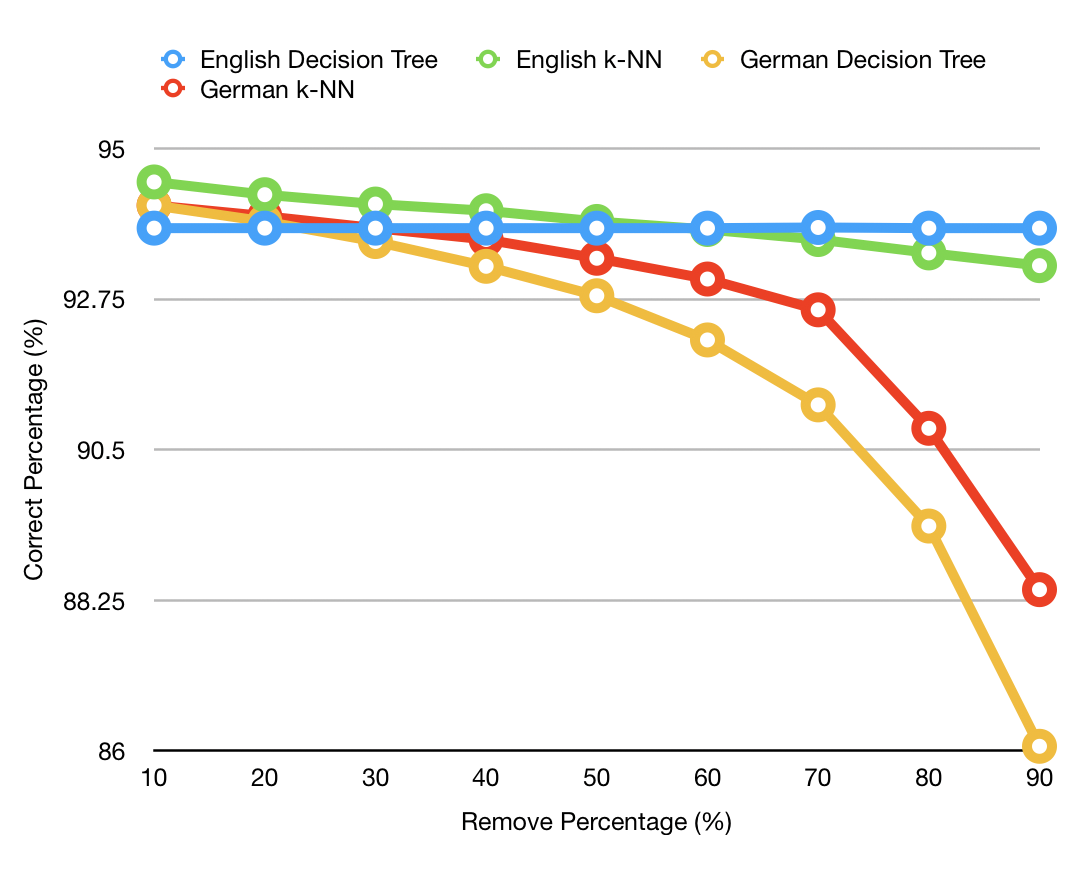
\includegraphics[width=0.5\textwidth]{images/performance_chart.png}
    \caption{Learning Curves for Different Sizes of Data}
\end{figure}

Despite the unchanged English decision tree result (it is a pruned tree and we have seen why it remains unchanged all the way above.), from above we can see obviously in all of the cases the more training data preserved the better the classification result is. But the percentage of correctly classified data in German nouns dropped much quicker than English verbs, especially in the decision tree classifier. I wounder if that suggests the smaller the data set is the more linear its learning curve is. I have taken a small step but the result was even more dramatic. Hence I believe the size of the data might not be the main reason of whether the learning curve is a linear one or a non-linear one, instad the fact the the German noun data is a balanced one (80\% of the data instances all in the top 4 classes) might be. 

\begin{figure}[h]
    \centering
    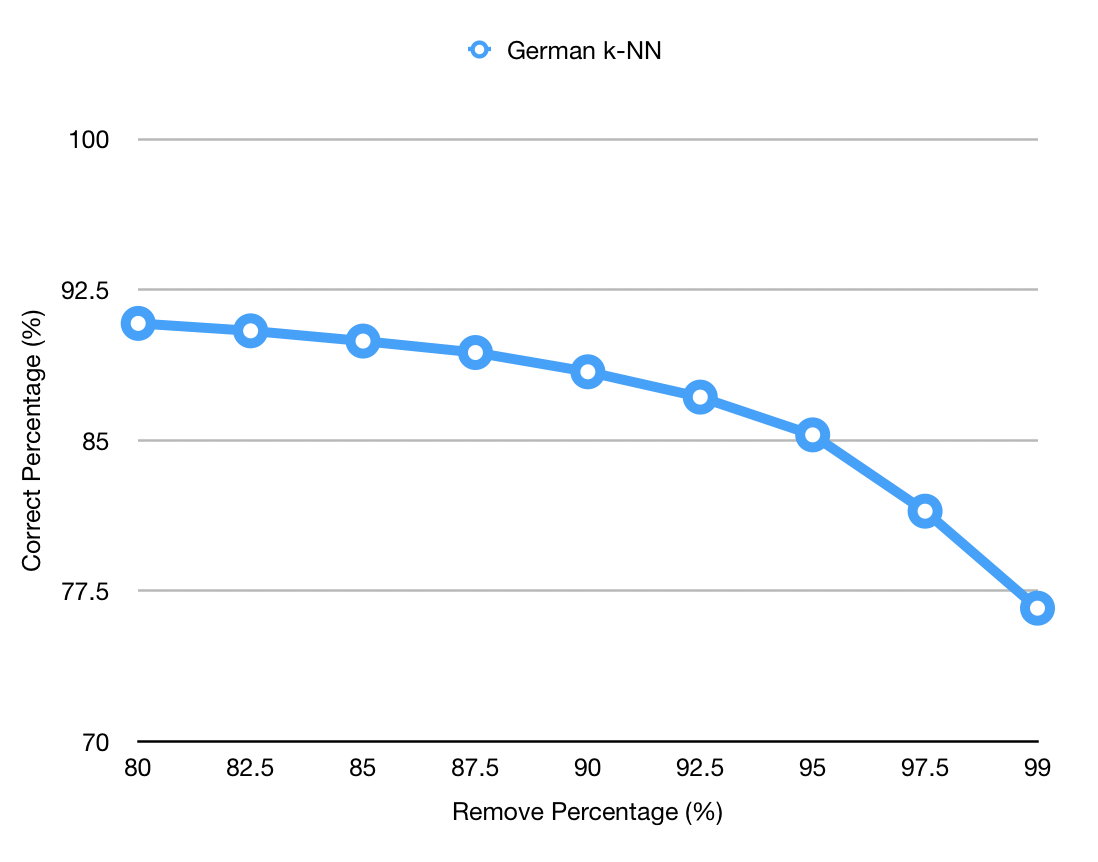
\includegraphics[width=0.5\textwidth]{images/performance_chart_2.png}
    \caption{Learning Curves for Small Sizes of Data of German nouns}
\end{figure}

Anyway, in order to find the best possible hyperparameter combinations, I first tried to increase the $k$ value from 1 to 10, as well as some large values like 20 and 50. Sadly none of them could increase the accuracy, it just kept going down as the $k$ increases. Modifying the nearest neighbour searching algorithm or distance weighing also didn't work. I would say the default hyperparameters are the best hyperparameters.

\end{document}